\newpage
\section{System Architecture}

The system functions are all represented here. The main one is “Taking pictures of the forest”, which is the main purpose of the system. All the other functions are made to serve this function.
\\
The system can be divided in sub-systems, which are:
\begin{itemize}[label=\textbullet]
    \item The protective case
    \item The power supply system
    \item The camera
    \item The microcontroller
    \item The shutter
    \item The storage system
    \item The sensors
\end{itemize}


\begin{figure}[!h]
    \centering
    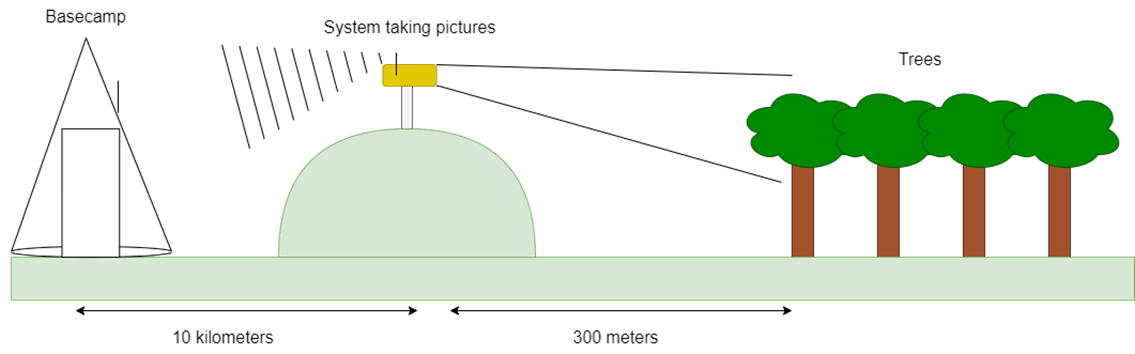
\includegraphics[width=0.95\textwidth]{\currfiledir/figures/shema_global.png}
    \caption{Schematic showing the global system installed in the forest}
\end{figure}
\tab \tab 

\newpage
\subsection{The camera}
The camera is a Lumix DMC-G5. This model has been used in a similar project called micrObs to take pictures of penguins in Antarctica. In this project, the camera has successfully been retro engineered in order to control it automatically. The system to control the camera is explained in the 3.5. part.

\begin{figure}[!h]
    \centering
    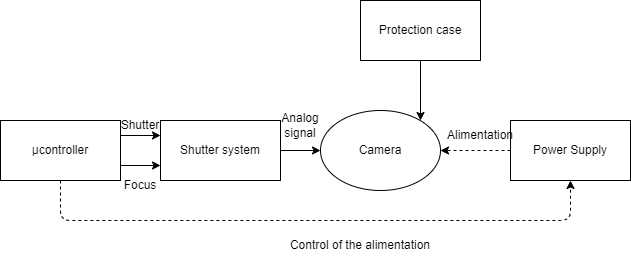
\includegraphics[width=0.9\textwidth]{\currfiledir/figures/camera_diagram.png}
    \caption{Architecture of the system surrounding the camera}
\end{figure}

The camera need a lens to be mounted on it in order to make it work properly. The calculations realized show the lens should be a lens with a focal length between 45 and 150 mm.

Here is the calculation:

\begin{figure}[!h]
    \centering
    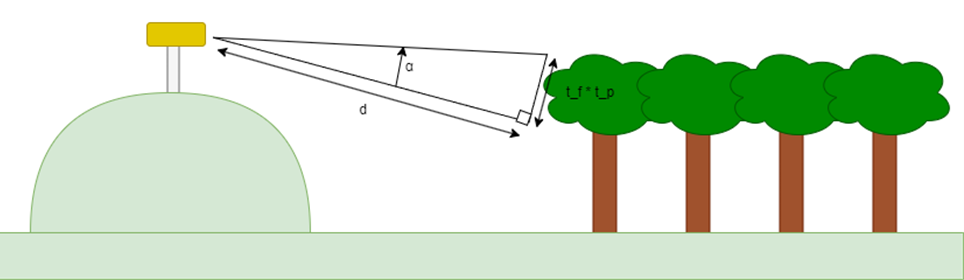
\includegraphics[width=0.85\textwidth]{\currfiledir/figures/calculation_schema.png}
    \caption{Schematic to calculate the focal length for the camera.}
\end{figure}

\noindent\(\alpha\): lens angle of the field of a (to calculate)\\
\(d\): distance between our system and trees (equal to 300 metres)\\
\(t_f\): size of a leaf, estimated to be 5,5 centimetres.\\
\(t_p\): height of the image, which corresponds to 1024 pixels.\\

\noindent According to the trigonometric formulas: \(\alpha=arctan\left(\frac{t_f*t_p}{d}\right)=32,4\textdegree\)

\newpage
%Schematic of different focal lengths
\begin{figure}[!h]
    \centering
    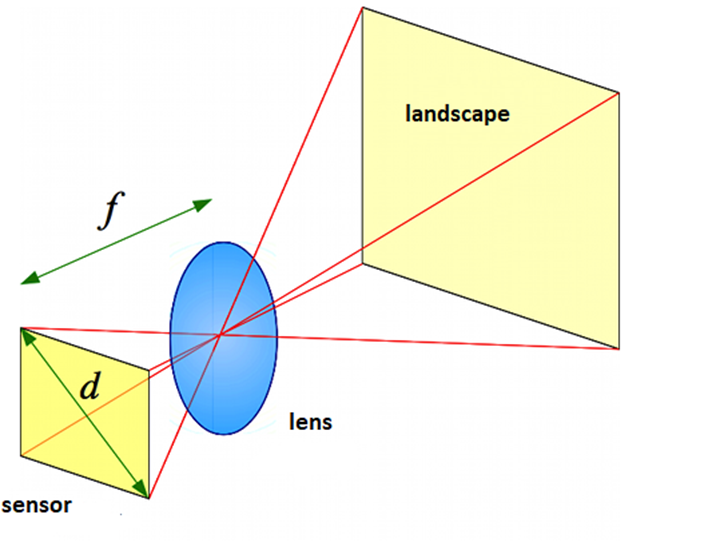
\includegraphics[width=0.75\textwidth]{\currfiledir/figures/calculation.png}
    \caption{Link between angle of view and focal length}
    \cite{focal_length}
\end{figure}

The field of view angle \((\alpha\)) horizontally, corresponding to the length (L) of the sensor, is given by the following formula:
% f=L/(2*tan⁡(α/2) )
\begin{equation}
    f=\frac{L}{2*tan\left(\frac{\alpha}{2}\right)}
\end{equation}

\noindent Where:\\
L: length of the sensor in mm\\
f: focal distance of the lens in mm\\
\(\alpha\): lens angle of the field of view\\
It is obtained: f = 117 mm\\

The equivalent focal length of a Micro 4/3 lens with a field of view of 32.4 degrees is approximately 117 mm.\\


\noindent According to the graph above, we should choose a lens between 100 and 200 mm. The smaller the angle of view (high focal length), the greater the magnification (long focal lengths will give the impression of being closer to the scene captured).\\
Our goal is not to visualize each leaf but each branch so a lens with a focal length of 175 mm will be sufficient for our project.\\
We have therefore selected this objective: \url{https://www.m43lenses.com/panasonic-45-175mm-f4-5.6/}
\newpage
\subsection{Use case}

% \begin{figure}[!h]
%     \centering
%     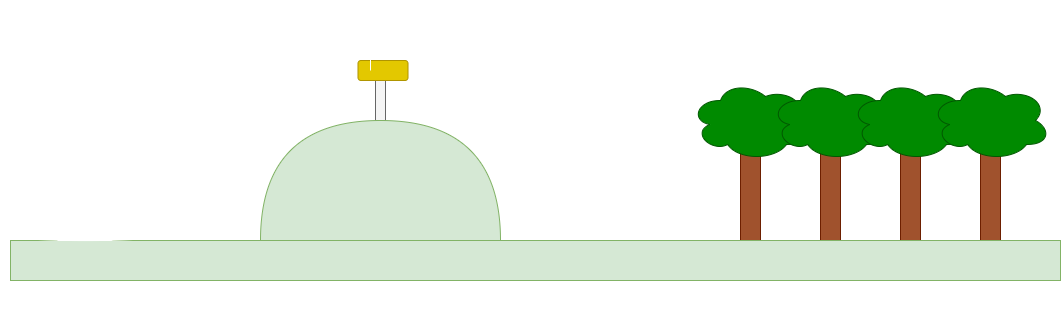
\includegraphics[width=1\textwidth]{\currfiledir/figures/use_case.png}
%     \caption{Use case of the system}
%     \label{fig:forest2}
% \end{figure}


The use case would be as following:
The researchers come once to install the system on a pole on a hill, in front of the group of trees they want to observe. The system would then be placed in the desired location within the forest. The system would be sending data to researchers to ensure that it is functioning properly and that the pictures being taken are of high quality. After 3 months, the researchers would return to the forest to retrieve the system, the stored pictures, and logs about the system state. Then, the researchers would be able to analyse the images.


\newpage
\begin{figure}[!h]
    \centering
    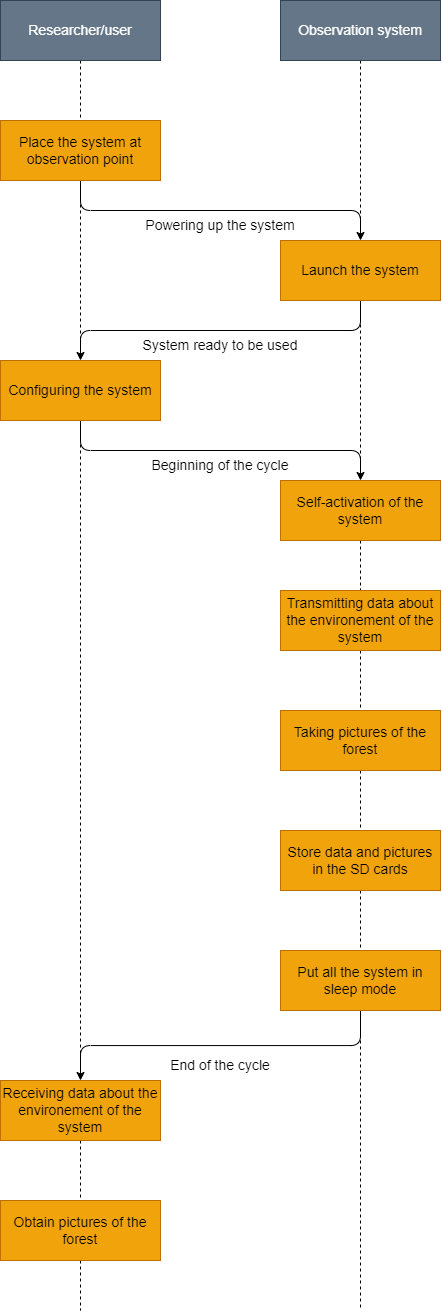
\includegraphics[height=0.95\textheight]{\currfiledir/figures/usage_scenario.png}
    \caption{Picture representing the intended usage scenario for the system.}
\end{figure}

\newpage
%début et titre de la sous-section
\subsection{The protective case}

\begin{figure}[!h]
    \centering
    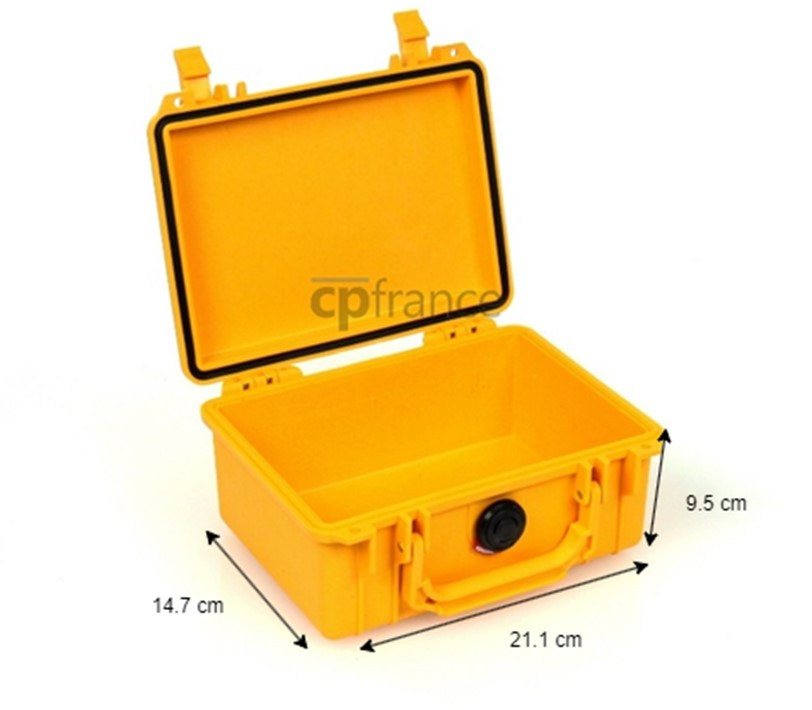
\includegraphics[width=0.8\textwidth]{\currfiledir/figures/case.jpg}
    \caption{Valise Peli™ 1150}
    \cite{case}
\end{figure}

The protective case has a role of protecting the whole system from the outside elements. The housing of the recording system needs to withstand extreme weather conditions, such as high temperatures (which can reach up to 35°C in Gabon), high humidity (up to 90\%), rain, and potential animal interference. To reduce wind-induced vibrations, a small plastic housing with a rubber seal was chosen (Protector 1150, Peli) to hold the camera, control unit, and GPS receiver.
\newpage

\subsection{Functional specifications}

\begin{figure}[!h]
    \centering
    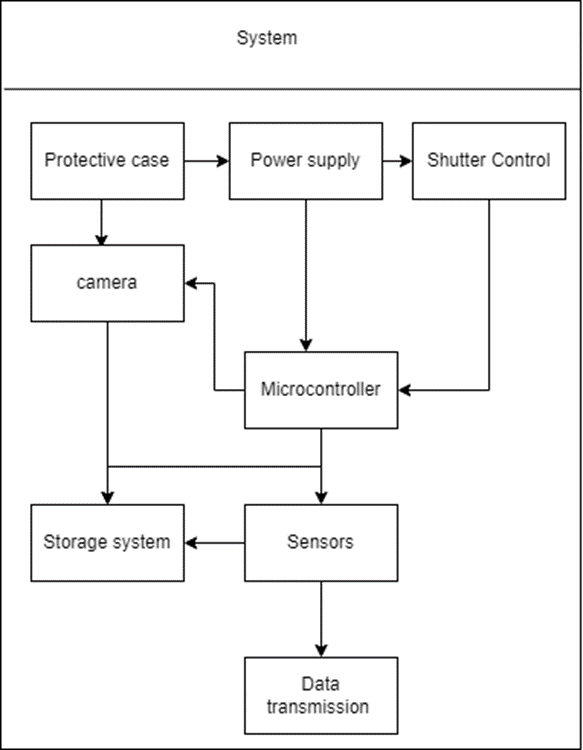
\includegraphics[height=0.5\textheight]{\currfiledir/figures/system.png}
    \caption{Schematic showing different functions interacting inside of the system}
\end{figure}

The diagram illustrates the interconnectivity of these functions, highlighting the relationships and data flow between them. To create a functional system, it is important to ensure that these components are properly integrated and configured to meet the specified technical requirements.

\newpage
\begin{table}[!h]
	\centering
	\begin{tabular}{|c|c|c|c|c|c|}
		\hline
		\rowcolor[HTML]{BFBFBF}
		x                                                  &
		Function                                           &
		Sub-function                                       &
		Criterion                                          &
		Value                                              &
		Flexibility                                          \\ \hline
		F1                                                 &
		\cellcolor[HTML]{CC99FF}Take photos                &
		                                                   &
		                                                   &
		                                                   &
		\cellcolor[HTML]{FFFFFF}{\color[HTML]{FFFFFF} }      \\ \hline
		F1.1                                               &
		                                                   &
		\cellcolor[HTML]{8EA9DB}\begin{tabular}[c]{@{}c@{}}Internal camera \\settings\end{tabular}  &
		                                                   &
		                                                   &
		\\ \hline
		C1.1.1                                             &
		                                                   &
		                                                   &
		\cellcolor[HTML]{A9D08E}Frequency                  &
		\cellcolor[HTML]{FFD966}Once                       &
		\cellcolor[HTML]{ED7D31}2                            \\ \hline
		F1.2                                               &
		                                                   &
		\cellcolor[HTML]{8EA9DB}\begin{tabular}[c]{@{}c@{}}Taking\\ photos regularly\end{tabular}  &
		                                                   &
		                                                   &
		\\ \hline
		C1.2.1                                             &
		                                                   &
		                                                   &
		\cellcolor[HTML]{A9D08E}Frequency                  &
		\cellcolor[HTML]{FFD966}\begin{tabular}[c]{@{}c@{}}2 times a\\ day\end{tabular}  &
		\cellcolor[HTML]{ED7D31}0                            \\ \hline
		F1.3                                               &
		                                                   &
		\cellcolor[HTML]{8EA9DB}\begin{tabular}[c]{@{}c@{}}Taking high-\\ quality photos\end{tabular}  &
		                                                   &
		                                                   &
		\\ \hline
		C1.3.1                                             &
		                                                   &
		                                                   &
		\cellcolor[HTML]{A9D08E}Resolution                 &
		\cellcolor[HTML]{FFD966}1920x1080                    &
		\cellcolor[HTML]{ED7D31}0                            \\ \hline
		C1.3.2                                             &
		                                                   &
		\multicolumn{1}{l|}{}                              &
		\cellcolor[HTML]{A9D08E}Distance                   &
		\cellcolor[HTML]{FFD966}\begin{tabular}[c]{@{}c@{}}300 meters\end{tabular}  &
		\cellcolor[HTML]{ED7D31}0                            \\ \hline
		C1.3.3                                             &
		                                                   &
		\multicolumn{1}{l|}{}                              &
		\cellcolor[HTML]{A9D08E}Fields of view             &
		\cellcolor[HTML]{FFD966}\begin{tabular}[c]{@{}c@{}}32.4°\end{tabular}  &
		\cellcolor[HTML]{ED7D31}1                            \\ \hline 
		F2                                                 &
		\cellcolor[HTML]{CC99FF}\begin{tabular}[c]{@{}c@{}}Possessing an extended\\ battery life\end{tabular}  &
		                                                   &
		                                                   &
		                                                   &
		\\ \hline
		F2.1                                               &
		                                                   &
		\cellcolor[HTML]{8EA9DB}\begin{tabular}[c]{@{}c@{}}Possessing an extended \\battery life\end{tabular}  &
		                                                   &
		                                                   &
		\\ \hline
		C2.1.1                                             &
		                                                   &
		                                                   &
		\cellcolor[HTML]{A9D08E}\begin{tabular}[c]{@{}c@{}}Desired uptime\end{tabular}  &
		\cellcolor[HTML]{FFD966}\(\approx\) 1 year                   &
		\cellcolor[HTML]{ED7D31}1                            \\ \hline
		F3                                                 &
		\cellcolor[HTML]{CC99FF}Storing data               &
		                                                   &
		                                                   &
		                                                   &
		\\ \hline
		F3.1                                               &
		                                                   &
		\cellcolor[HTML]{8EA9DB}Store photos               &
		                                                   &
		                                                   &
		\\ \hline
		C3.1.1                                             &
		                                                   &
		                                                   &
		\cellcolor[HTML]{A9D08E}\begin{tabular}[c]{@{}c@{}}Picture-dedicated \\storage space\end{tabular}  &
		\cellcolor[HTML]{FFD966}\textgreater 16 Go         &
		\cellcolor[HTML]{ED7D31}1                            \\ \hline
		F3.2                                               &
		                                                   &
		\cellcolor[HTML]{8EA9DB}\begin{tabular}[c]{@{}c@{}}Storing  \\ information on \\ the device state\end{tabular} &
		                                                   &
		                                                   &
		\\ \hline
		C3.2.1                                             &
		                                                   &
		                                                   &
		\cellcolor[HTML]{A9D08E}\begin{tabular}[c]{@{}c@{}}Information-dedicated \\ storage  \\ space\end{tabular} &
		\cellcolor[HTML]{FFD966}16 Mo                      &
		\cellcolor[HTML]{ED7D31}3                            \\ \hline
		C3.2.2                                             &
		                                                   &
		                                                   &
		\cellcolor[HTML]{A9D08E}\begin{tabular}[c]{@{}c@{}}Logging period\end{tabular} &
		\cellcolor[HTML]{FFD966}\(\approx\) 1 months                 &
		\cellcolor[HTML]{ED7D31}3                            \\ \hline
		F4                                                 &
		\cellcolor[HTML]{CC99FF}\begin{tabular}[c]{@{}c@{}}Conveying system \\status information\end{tabular} &
		                                                   &
		                                                   &
		                                                   &
		\\ \hline
		F4.1                                               &
		                                                   &
		\cellcolor[HTML]{8EA9DB}Collecting information             &
		                                                   &
		                                                   &
		\\ \hline
		C4.1.1                                             &
		                                                   &
		                                                   &
		\cellcolor[HTML]{A9D08E}\begin{tabular}[c]{@{}c@{}}Remaining battery\\charge percentage\end{tabular} &
		\cellcolor[HTML]{FFD966}\begin{tabular}[c]{@{}c@{}}Error margin \\ of 10\%\end{tabular} &
		\cellcolor[HTML]{ED7D31}2                            \\ \hline
	\end{tabular}
\end{table}

\newpage

% Please add the following required packages to your document preamble:
% \usepackage{multirow}
% \usepackage[table,xcdraw]{xcolor}
% If you use beamer only pass "xcolor=table" option, i.e. \documentclass[xcolor=table]{beamer}
% Please add the following required packages to your document preamble:
% \usepackage{multirow}
% \usepackage[table,xcdraw]{xcolor}
% If you use beamer only pass "xcolor=table" option, i.e. \documentclass[xcolor=table]{beamer}
\begin{table}[!h]
    \centering
    \begin{tabular}{|c|c|c|c|c|c|}
    \hline
     &
       &
       &
      \cellcolor[HTML]{A9D08E} &
      \cellcolor[HTML]{FFD966}\begin{tabular}[c]{@{}c@{}}0°C to 5\\ 0°C\end{tabular} &
      \cellcolor[HTML]{ED7D31}2 \\ \cline{5-6} 
    \multirow{-2}{*}{C4.1.2} &
      \multirow{-2}{*}{} &
      \multirow{-2}{*}{} &
      \multirow{-2}{*}{\cellcolor[HTML]{A9D08E}Temperature} &
      \cellcolor[HTML]{FFD966}\begin{tabular}[c]{@{}c@{}}Precision \\ of 1°C\end{tabular} &
      \cellcolor[HTML]{ED7D31}0 \\ \hline
    C4.1.3 &
       &
       &
      \cellcolor[HTML]{A9D08E}Humidity &
      \cellcolor[HTML]{FFD966}\begin{tabular}[c]{@{}c@{}}80 to \\ 100\%\end{tabular} &
      \cellcolor[HTML]{ED7D31}2 \\ \hline
    C4.1.4 &
       &
       &
      \cellcolor[HTML]{A9D08E}\begin{tabular}[c]{@{}c@{}}Remaining\\  storage\\  space\end{tabular} &
      \cellcolor[HTML]{FFD966}\begin{tabular}[c]{@{}c@{}}Warning \\ at 90\%\end{tabular} &
      \cellcolor[HTML]{ED7D31}2 \\ \hline
    C4.1.5 &
       &
       &
      \cellcolor[HTML]{A9D08E}\begin{tabular}[c]{@{}c@{}}Device \\ motion\end{tabular} &
      \cellcolor[HTML]{FFD966}\begin{tabular}[c]{@{}c@{}}Precision : \\ ± 1cm | \\ ± 1°\end{tabular} &
      \cellcolor[HTML]{ED7D31}1 \\ \hline
    F4.2 &
       &
      \cellcolor[HTML]{8EA9DB}\begin{tabular}[c]{@{}c@{}}Transmitting \\ data remotely\end{tabular} &
       &
       &
       \\ \hline
    C4.2.1 &
       &
       &
      \cellcolor[HTML]{A9D08E}Range &
      \cellcolor[HTML]{FFD966}\(\geq\) 10km &
      \cellcolor[HTML]{ED7D31}1 \\ \hline
    F5 &
      \cellcolor[HTML]{CC99FF}\begin{tabular}[c]{@{}c@{}}Working in a\\  specific \\ environment\end{tabular} &
       &
       &
       &
       \\ \hline
    F5.1 &
       &
      \cellcolor[HTML]{8EA9DB}\begin{tabular}[c]{@{}c@{}}Resisting Central \\ African climate\end{tabular} &
       &
       &
       \\ \hline
    C5.1.1 &
       &
       &
      \cellcolor[HTML]{A9D08E}\begin{tabular}[c]{@{}c@{}}Humidity \\ and fog\end{tabular} &
      \cellcolor[HTML]{FFD966}\begin{tabular}[c]{@{}c@{}}\textgreater 90\% of \\ humidity\end{tabular} &
      \cellcolor[HTML]{ED7D31}0 \\ \hline
    C5.1.2 &
       &
       &
      \cellcolor[HTML]{A9D08E}Temperature &
      \cellcolor[HTML]{FFD966}20°C to 35°C &
      \cellcolor[HTML]{ED7D31}0 \\ \hline
    C5.1.3 &
       &
       &
      \cellcolor[HTML]{A9D08E}Rain &
      \cellcolor[HTML]{FFD966}\begin{tabular}[c]{@{}c@{}}equivalent to\\ IPX4\end{tabular} &
      \cellcolor[HTML]{ED7D31}0 \\ \hline
    \cellcolor[HTML]{FFFFFF}F5.2 &
      \cellcolor[HTML]{FFFFFF} &
      \cellcolor[HTML]{8EA9DB}Size &
       &
       &
       \\ \hline
    \cellcolor[HTML]{FFFFFF}C5.2.1 &
      \cellcolor[HTML]{FFFFFF} &
       &
      \cellcolor[HTML]{A9D08E}Dimensions &
      \cellcolor[HTML]{FFD966}200x300x150 mm &
      \cellcolor[HTML]{ED7D31}2 \\ \hline
    \cellcolor[HTML]{FFFFFF}F5.3 &
      \cellcolor[HTML]{FFFFFF} &
      \cellcolor[HTML]{8EA9DB}Weight &
       &
       &
       \\ \hline
    \cellcolor[HTML]{FFFFFF}C5.3.1 &
      \cellcolor[HTML]{FFFFFF} &
       &
      \cellcolor[HTML]{A9D08E}Mass &
      \cellcolor[HTML]{FFD966}4 kg &
      \cellcolor[HTML]{ED7D31}1 \\ \hline
    \cellcolor[HTML]{FFFFFF}F5.4 &
      \cellcolor[HTML]{FFFFFF} &
      \cellcolor[HTML]{8EA9DB}\begin{tabular}[c]{@{}c@{}}Installation\end{tabular} &
       &
       &
       \\ \hline
    \cellcolor[HTML]{FFFFFF}C5.4.1 &
      \cellcolor[HTML]{FFFFFF} &
       &
      \cellcolor[HTML]{A9D08E}\begin{tabular}[c]{@{}c@{}}Relevant stand \\ or platform\end{tabular} &
      \cellcolor[HTML]{FFD966}??? &
      \cellcolor[HTML]{ED7D31}1 \\ \hline
    \end{tabular}
\end{table}
\tab\tab
\newpage
\subsection{The power supply system}

\begin{figure}[!h]
    \centering
    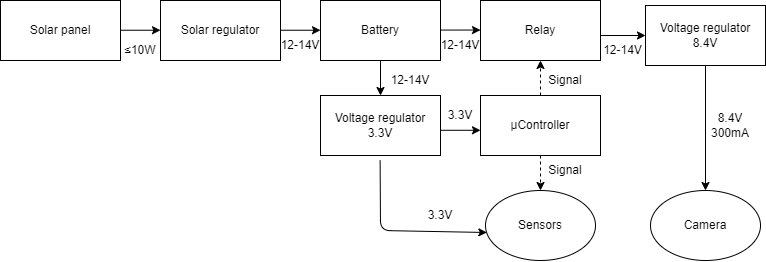
\includegraphics[width=0.8\textwidth]{\currfiledir/figures/alimentation_diagramme.png}
    \caption{Power supply architecture}
\end{figure}


\subsubsection{Camera and relay}
\begin{figure}[!h]
    \centering
    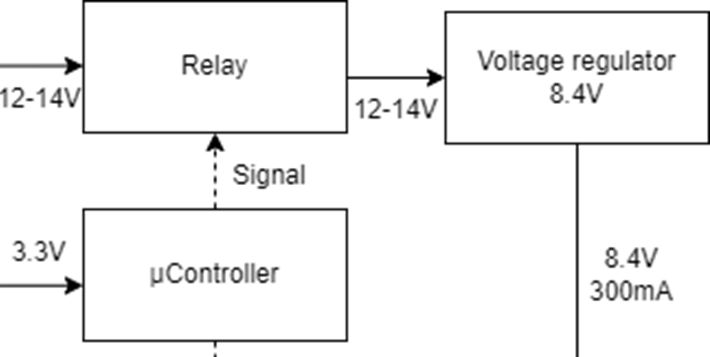
\includegraphics[width=0.5\textwidth]{\currfiledir/figures/camera_relay.png}
    \caption{Schematic showing the architecture of the camera and relay}
\end{figure}

The camera necessitates an 8.4V power supply and a current draw of 300mA for optimal operation. The system connects to the camera through a dummy battery featuring wired connections to the board. A relay, managed by the microcontroller, controls the camera's power supply. This approach is energy-efficient and offers low-power consumption. The relay consumes only 20mA of current when activated and no power when deactivated. Any relay with low power consumption operating at 3.3V is suitable for use.\\
To ensure voltage stability from the battery to the camera at 8.4V, a voltage regulator is placed after the relay. Installing the relay before the regulator helps avoid current loss within the regulator, enhancing the system's overall efficiency.



\begin{figure}[!h]
    \centering
    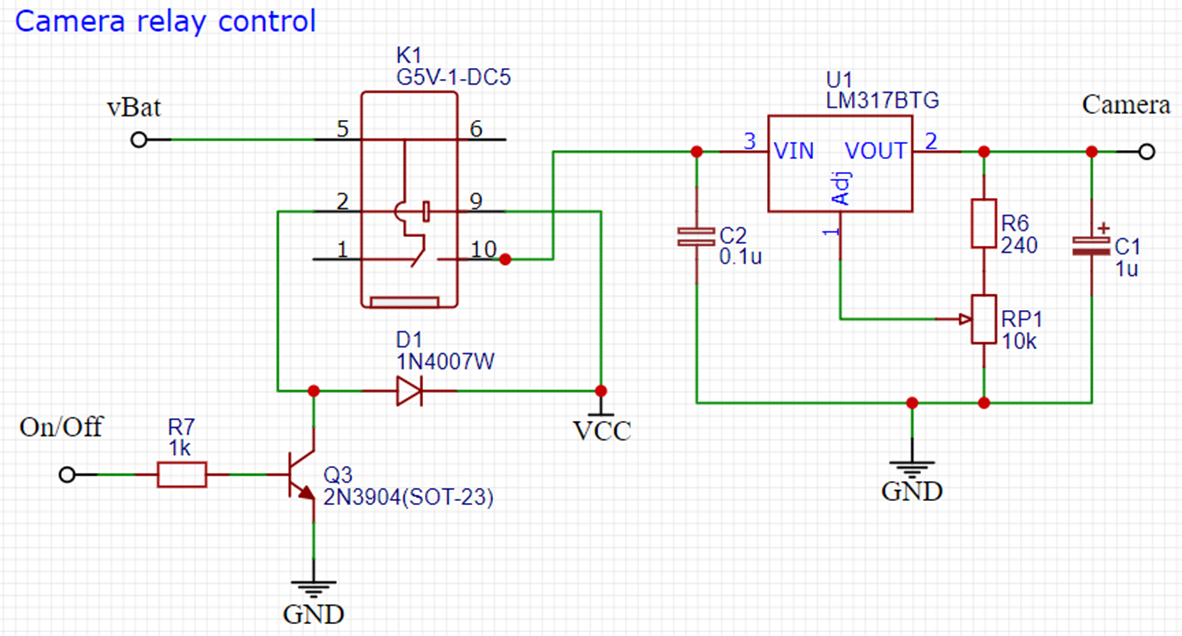
\includegraphics[width=1\textwidth]{\currfiledir/figures/relay.png}
    \caption{Camera-relay control}
\end{figure}

\newpage
\subsubsection{Battery and voltage regulator}

%Image avec sous figure
\begin{figure}[!h]
    \center{}
    %sous figure a
    \subfigure[Schematic showing the architecture of the regulator]{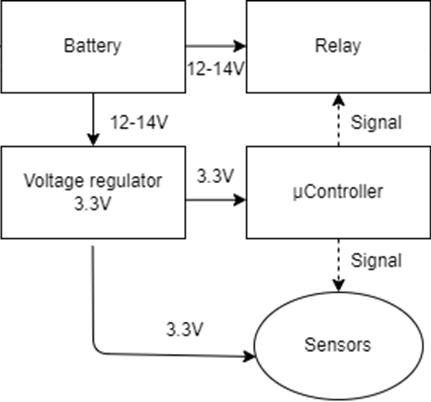
\includegraphics[width=0.4\textwidth]{\currfiledir/figures/regulator_33.png}}
    %sous figure b
    \subfigure[MT1763IS8 regulator]{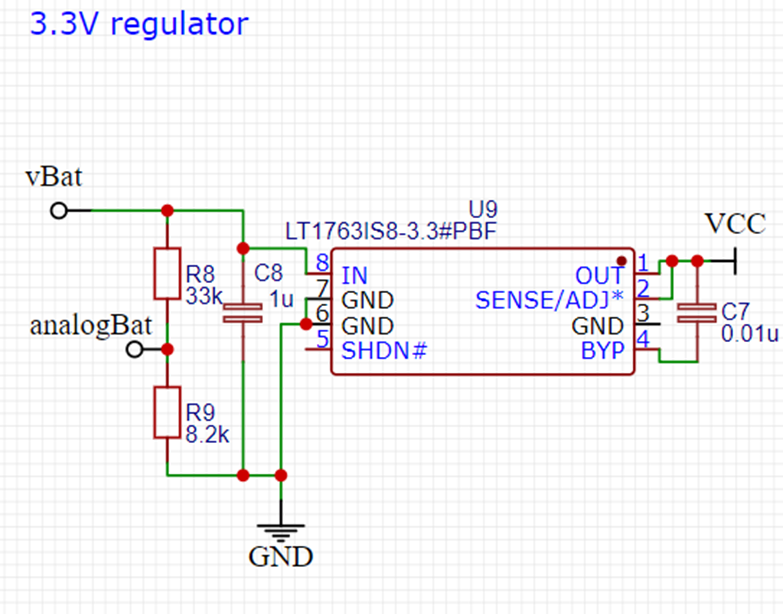
\includegraphics[width=0.59\textwidth]{\currfiledir/figures/regulator.png}}
    %légende de l'image
    % \caption{Exemple de sous-figure}
    %nom pour la citation de figure
\end{figure}
%fin de la figure

The LT1763IS8 is a voltage regulator designed to provide a stable 3.3V output while accepting an input voltage of up to 20V. It boasts a low quiescent current of 30µA, ensuring minimal power loss when supplying high output current, with less than 1mA lost to ground. Capable of delivering a maximum output current of 500mA, the LT1763IS8 is an efficient and reliable choice for regulating voltage in our application.

\newpage
\subsubsection{Sensors}
The system incorporates an array of low-power sensors, powered by a 3.3V voltage supply from the regulator, to ensure accurate and reliable measurements while maintaining low power consumption. These sensors are scheduled to collect data every 30 minutes and transmit the information through LoRa, with the exception of the motion sensor, which is read upon detecting an interruption. All data is also stored locally in a CSV format on a microSD card.\\
-	Motion Sensor: The ICM-20602 motion sensor operates in low power mode, consuming 1.33mA of current, and in Low-Noise mode, consuming 2.79mA. The primary purpose of the motion sensor is to detect when the container has been moved, which may cause the photos not to be aligned enough. When an interruption is detected, the motion sensor data, including rotation and acceleration, is read and transmitted through LoRa. The data format for motion is "date;gyro;acceleration".\\
-	Humidity/Temperature Sensor: The AM2320 sensor measures both humidity and external temperature, consuming 50µA in sleep mode and 1mA in active mode. The sensor reads data every 30 minutes and sends it through LoRa. The data format is "date;internal temperature;external temperature;humidity;light".\\
-	Internal Case Temperature Sensors: The LM35DZ sensors monitor the internal case temperature with a power consumption of less than 60µA. These sensors provide real-time data to the microcontroller.\\
-	Light Sensor: The TSL2561 light sensor operates with a power consumption of 2µA when turned down and a typical current of 0.24mA when active. This sensor measures ambient light levels every 30 minutes, and the light data is used to determine the lighting conditions when a photo is taken. If the light level at the scheduled photo-taking time is insufficient, the system will delay the photo-taking event until adequate lighting is available. The data format for this sensor is included in the combined format for the humidity/temperature sensor.\\
By using these low-power sensors, the system effectively minimizes energy consumption while still providing accurate and reliable measurements. All data, including sensor readings and motion events, is stored in a CSV format on a microSD card, ensuring that the information is readily available for analysis and review.

\subsubsection{Micro-controller}
The microcontroller used in the system is an STM32 Nucleo F303K8, which is powered at 3.3V directly from the voltage regulator. When active, with all peripherals disabled, it draws a current of 13mA. In sleep mode, with the Real-Time Clock (RTC) enabled, the microcontroller consumes only 3mA. It can be activated either by the interrupt signal from the motion detector or by the RTC at a predefined time, ensuring efficient power management and prolonging battery life while maintaining the responsiveness of the system. The STM32 Nucleo F303K8 offers flexible power options and low-power modes, making it suitable for energy-conscious applications that require optimal performance.

\newpage
% Solar panel and regulator
\subsubsection{Solar panel and regulator}
The primary power source for the system is a 12V 2.3Ah (27.6Wh) lead battery, chosen for its high capacity, its ability to retain charge over extended periods and its ability to resist to high temperatures. With an average power consumption of 127mAh a day, the battery can supply power up to 18 days.

\begin{table}[!h]
    \centering
    \begin{tabular}{|c|c|c|c|}
    \hline
     &
      \begin{tabular}[c]{@{}c@{}}Time where the system \\ is on per day(s)\end{tabular} &
      Current &
      \begin{tabular}[c]{@{}c@{}}Average consumption \\ per days (mAh)\end{tabular} \\ \hline
    Camera                     & 20    & 330 & 1,8333 \\ \hline
    Sensors                    & 480   & 50  & 6,6666 \\ \hline
    Sleep mode                 & 85900 & 5   & 119,30 \\ \hline
    Total consumption per days &       &     & 127,81 \\ \hline
    \end{tabular}
\end{table}

A 10W solar panel with 23\% efficiency is employed in this system to provide a significant safety margin, considering the intermittent nature of solar energy that can sometimes generate no power during the day. The solar panel is responsible for charging the lead battery during sunlight hours. A solar voltage regulator ensures that the voltage from the solar panel is within the appropriate range for charging the lead battery. The battery can be fully recharged with 2 days of sunshine.


\begin{figure}[!h]
    \centering
    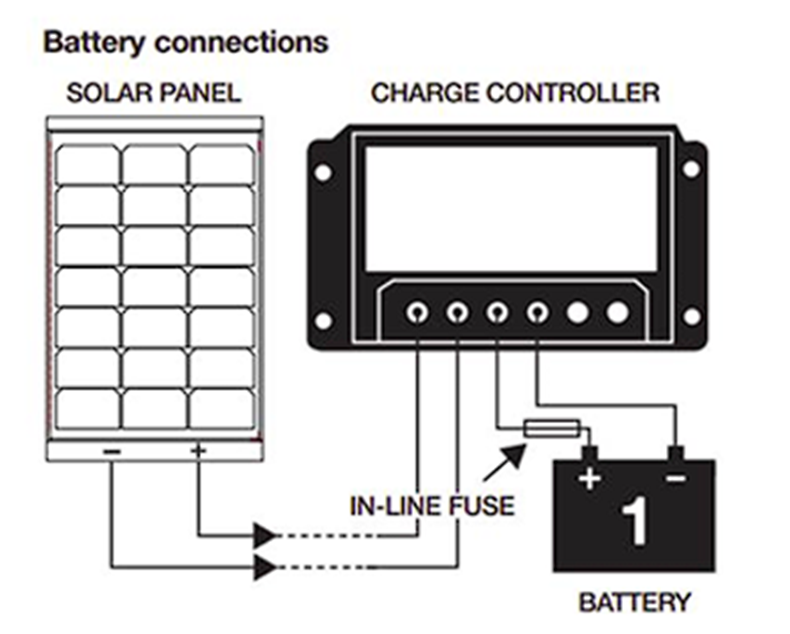
\includegraphics[width=0.8\textwidth]{\currfiledir/figures/battery_connection.png}
    \caption{Battery connection}
    \cite{battery}
\end{figure}

The solar panel and the battery are directly connected to the charge controller. The charge controller uses PWM to charge the battery with the good power.
\newpage
\subsection{The microcontroller}

\begin{figure}[!h]
    \centering
    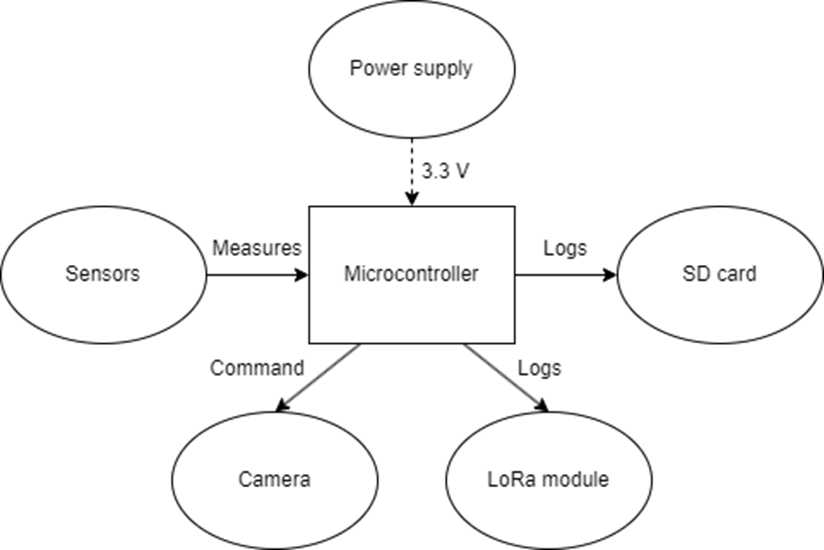
\includegraphics[width=0.8\textwidth]{\currfiledir/figures/micro.png}
    \caption{Schematic of the microcontroller and its relationships with other elements}
\end{figure}

The microcontroller is the core of the device. It is responsible to command the whole system. The STM32 Nucleo F303K8 microcontroller was chosen for this project due to several key features that make it suitable for our application. Firstly, it has very low power consumption, with only 3mA in sleep mode and 13mA during operation. Secondly, it includes a built-in Real-Time Clock (RTC), eliminating the need for an external RTC module, thereby saving cost and board space. Furthermore, one was readily available, which saved time and reduced the overall project cost.\\
The microcontroller operates on a 3.3V power supply, a common voltage level for many electronic devices, simplifying integration into our project without the need for additional voltage regulation or level shifting circuits. This compatibility allows for seamless connections with the various sensors in our system, such as the ICM-20602 motion sensor, the AM2320 humidity and temperature sensor, the LM35DZ internal case temperature sensors, and the TSL2561 light sensor. The microcontroller receives data from these sensors and processes it to make decisions and execute predefined actions, ensuring the proper functioning of the system.\\
Lastly, the STM32 Nucleo F303K8 microcontroller offers multiple communication interfaces, such as I2C, SPI, and UART, providing flexibility in connecting and communicating with the sensors and other peripherals, like the LoRa module, in our project. These interfaces facilitate the efficient transmission of sensor data to the microcontroller for real-time monitoring, analysis, and response.\\
The microcontroller is being programmed in order to use the temperature and humidity sensor, and the SD card in order to create logs.

\newpage
\subsection{The shutter system}
\label{shutter}
The shutter system is a sub-system allowing the microcontroller to command the camera. This system was developed with the help of video tutorials dismantling commercial remote shutters, showing that they were mainly made of resistances.
%Schematic of the shutter system
\begin{figure}[!h]
    \centering
    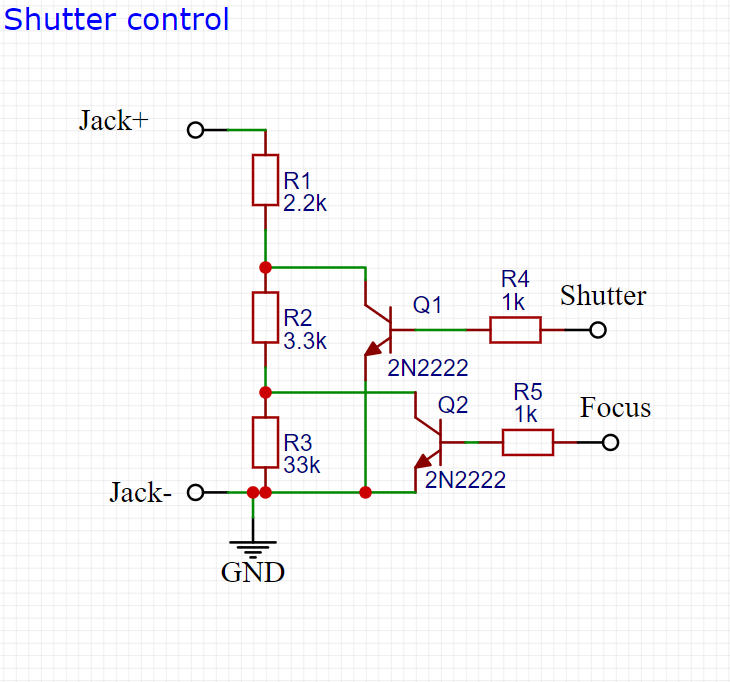
\includegraphics[width=0.7\textwidth]{\currfiledir/figures/shutter.png}
    \caption{Schematic of the shutter system}
    \cite{JACK}
\end{figure}

\begin{figure}[!h]
    \centering
    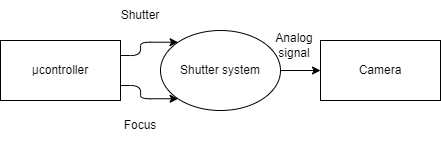
\includegraphics[width=0.9\textwidth]{\currfiledir/figures/shutter_diagram.png}
    \caption{Shutter system}
\end{figure}

The system is made of a jack socket, connected to resistances. The shutter and the focus pin are linked to the microcontroller. The microcontroller can then be programmed to put the pins at a high or a low state to trigger the shutter or the focus of the camera. By controlling transistor, the camera sees a change in the resistor and trigger the associated actions.
\newpage
\subsection{LoRa}
LoRa is a wireless communication protocol that is designed for long-range, low-power, and low-data-rate applications. LoRa is based on chirp spread spectrum modulation (CSS) technology, which enables long-range communication with low power consumption, making it suitable for IoT devices that need to transmit data over long distances while consuming minimal power.

\begin{figure}[!h]
    \centering
    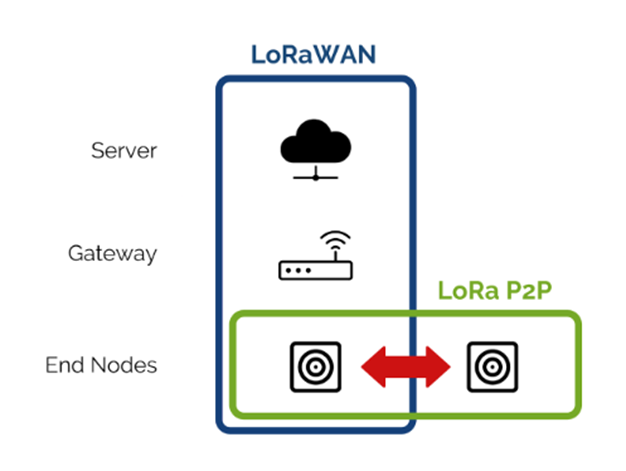
\includegraphics[width=0.8\textwidth]{\currfiledir/figures/lora_P2P.png}
    \caption{LoRa WAN and LoRa P2P scheme}
\end{figure}

LoRa is primarily designed for long-range communication between IoT devices and gateways using a star network topology. However, it is possible to use LoRa for peer-to-peer (P2P) communication between two LoRa devices without the need for a gateway or network server.
This type of communication becomes important and applicable because the remote monitoring system, to which the LoRa protocol will be applied, is located in a forest. Where there is no internet connection.


%3.6.1	Analysis and expressions of needs for LoRa
\subsubsection{Analysis and expressions of needs for LoRa}
The analysis and expression of needs would involve identifying the specific requirements for LoRa. For this, it is considered two main needs. The first is to establish communication between the transmitter and the receiver. The second is to cover a distance greater than or equal to 10 km. The goal is to send data via LoRa protocol, obtained by the sensors connected to the remote monitoring system, directly to the site where researchers will be able to analyse the information about its operation.

\newpage
%3.6.2	Use case for LoRa
\subsubsection{Use case for LoRa}
The system would then be placed in the desired location within the forest. For this reason, LoRa peer-to-peer communication will be used, as there is no internet connection in the location mentioned. All operating data obtained by the monitoring system will be passed to the LoRa transmitter via the microcontroller. With this, the data sent should reach the receiver located at a distance of 10 km or more. Finally, with the communication effected, the researchers will be able to analyze the operating conditions of the system.  In our case, the architecture is organized like this:
\begin{figure}[!h]
    \centering
    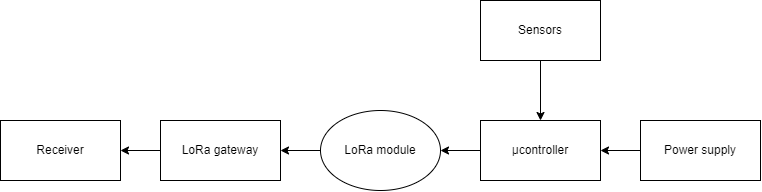
\includegraphics[width=1\textwidth]{\currfiledir/figures/lora_diagram.png}
    \caption{LoRa architecture diagram}
\end{figure}

\newpage
%4.6.4	Technical constraints
\subsubsection{Technical constraints}
%Graph presenting the different elements exercising constraints on the LoRa
\begin{figure}[!h]
    \centering
    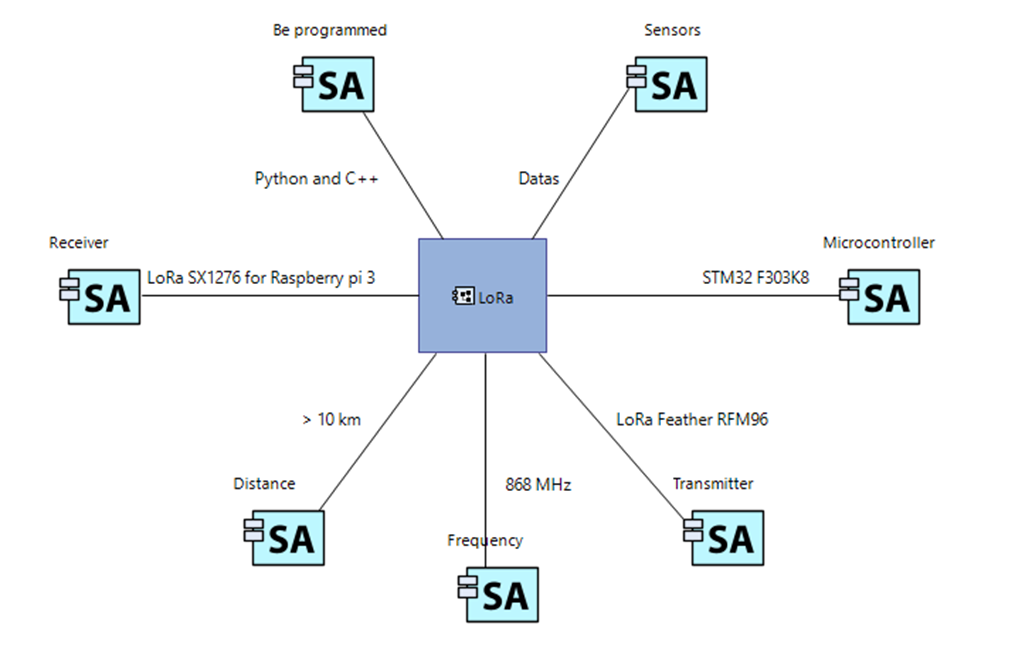
\includegraphics[width=0.90\textwidth]{\currfiledir/figures/lora_constraint.png}
    \caption{Graph presenting the different elements exercising constraints on the LoRa}
\end{figure}

%bold text "a"
\noindent\textbf{Sensors:} The sensors will be the source of the monitoring system's operational data, which will be sent for transmission via LoRa protocol.\\

\noindent\textbf{Microcontroller:} The microcontroller STM32 F303K8 will pass the data obtained from the sensors to the LoRa transmitter, so that this information can be sent to the receiver.\\

\noindent\textbf{Transmitter:} As a transmitter, the LoRa Feather RFM96 will be used, which will send the obtained data to the receiver.\\

\noindent\textbf{Frequency:} The frequency on which the LoRa communication will take place is 868 MHz.\\

\noindent\textbf{Distance:} Sending data must pass over a distance of 10 km or more.\\

\noindent\textbf{Receiver:} The Lora SX1276 connected to the raspberry pi 3 will be used as a receiver, which will act as a gateway allowing researchers to retrieve data from the monitoring system.\\

\noindent\textbf{Be programmed :}  In order for communication to take place, a code for sending data, in C++ language will be written in the LoRa transmitter connected to the microcontroller. For the receiver, a code in python will be written for retrieving the sent data.

%lora transmitter
\subsubsection{LoRa transmitter}
As transmitter the LoRa RFM95W module is used, which is connected to the STM32. The RFM95W module is based on the Semtech SX1276 chip, which is a high-performance, low-power LoRa transceiver. It operates in the 868 MHz and 915 MHz frequency bands, and provides a range of up to 5-10 km in open areas, depending on the transmit power and other environmental factors.
\begin{figure}[!h]
    \centering
    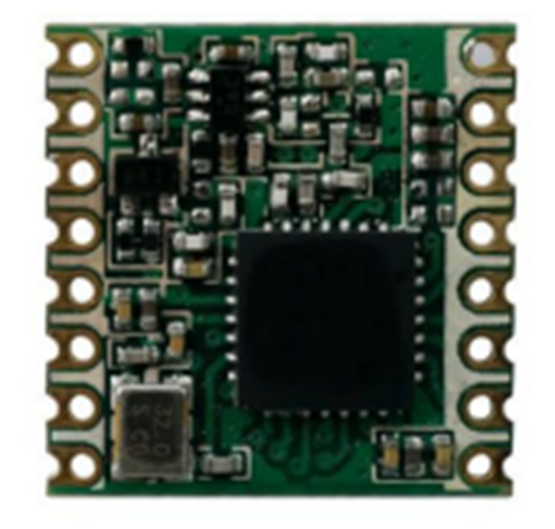
\includegraphics[width=0.50\textwidth]{\currfiledir/figures/RFM95W.png}
    \caption{LoRa RFM95W}
    \cite{RFM95W}
\end{figure}

Before configuring the LoRa module to act as a transmitter, it was necessary to connect a wire to the component in order to obtain an antenna. The size of the wire varies according to the transmission frequency. In this case for a frequency of 868 MHz, according to the manufacturer's website, the wire size is 8.2 cm. Because of this it was used.\\
Next, the Arduino IDE was used to configure and implement the C++ code, available for analysis in the appendix, for sending data via LoRa. The code was written with the help of existing Arduino libraries and forums on the subject available on the internet.

\newpage
%lora receiver
\subsubsection{LoRa receiver}
As receiver, the LoRa SX1276/ GPS Hat for Raspberry will be used. In this sense, the Raspberry pi 3 connected to the LoRa will have access to the received information. The currently available module for the project already has an uFL antenna.

\begin{figure}[!h]
    \centering
    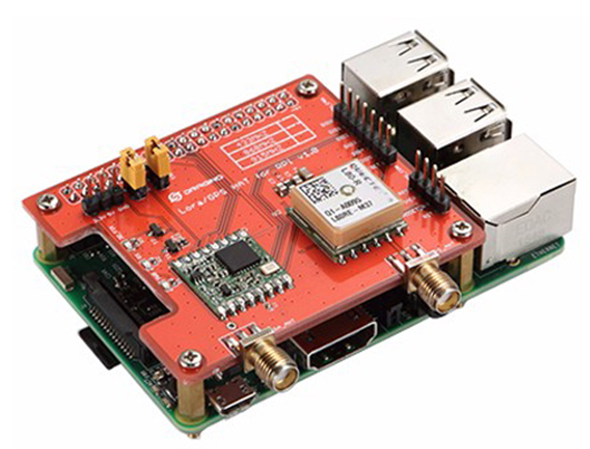
\includegraphics[width=0.60\textwidth]{\currfiledir/figures/lora_hat.png}
    \caption{LoRa/GPS HAT for Raspberry}
    \cite{Lora}
\end{figure}

The data received by Raspberry is automatically stored in a database available in a libre office Calc folder. This way, the user can have easy access to the system state.
For the Raspberry to work as a data receiver, it was necessary to configure it to enable some functions and update and download specific libraries for the LoRa SX1276. With this done, a program was written in python, available for analysis in the appendix, to receive the data. The data received by Raspberry is automatically stored in a database available in a libre office Calc folder. This way, the user can have easy access to the system state.\\

\begin{figure}
    \centering
    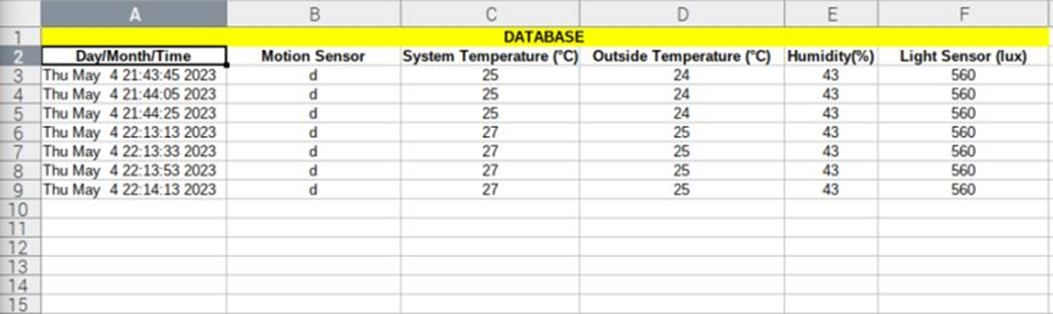
\includegraphics[width=0.8\textwidth]{\currfiledir/figures/lora_database.png}
    \caption{Sensors database}
\end{figure}

The database records the date and time each information is received. For the motion sensor, the letter "d" means that there is receiving data, if the system eventually moves, data about the movement will be sent, and letter "m" will appear in the database, indicating movement.


% \subsubsection{Tests to be performed for the LoRa communication system}
% The functional testing of the LoRa system will focus on two main aspects: communication between transmitter and receiver, and the maximum distance over which data can be sent.\\
% For the first one, through programming, a simple data transmission should be performed to the receiver using the LoRa transmitter. In this sense, a check of the received data should be made to see that no information has been lost.\\
% With the communication established, the test of the range of the transmission signal was performed. The transmitter was positioned on the second floor of the Les Roses building at approximately 230 m from the receiver, in the Fablab, at Polytech Vinci. An image representing the location and distance between the transmitter and receiver is shown below:\\
% \newpage
% \begin{figure}[!h]
%     \centering
%     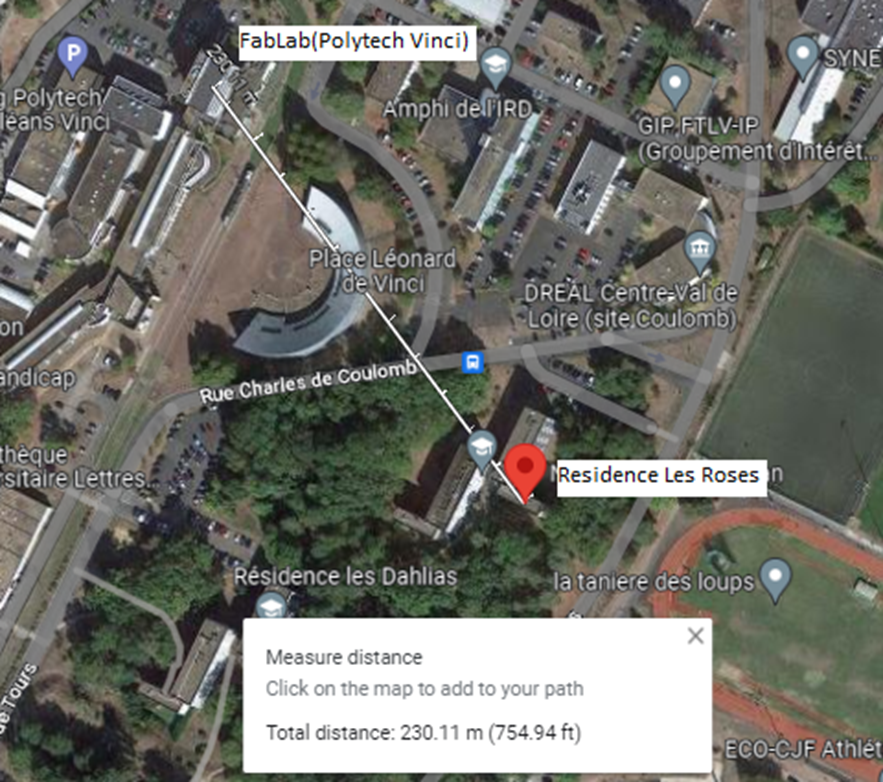
\includegraphics[width=0.60\textwidth]{\currfiledir/figures/map.png}
%     \caption{Location and distance between the transmitter and receiver.}
% \end{figure}

% Although the data was received in Raspberry, the signal was weak. The signal information is listed below:\\
% \tab •	Packet RSSI: -97\\
% \tab •	RSSI: -96\\
% \tab •	SNR: -8\\
% The factors that may have influenced this result are related, above all, to the transmission power and to the urban area noise that interferes with the signal quality.\\
% First, the antenna used for transmission is an 8.2 cm wire connected to the microcontroller. By replacing it with a more powerful model, it will be possible to send the signal over a longer distance.\\
% Next, the place where the transmission was made was not exactly the highest point of the building.\\
% Besides these factors, there is the fact that the signal suffers interference from urban noise, which affects the signal quality.\\
% Finally, in the transmission settings, the signal was sent with a Spreading factor SF=7, and it is possible to increase it up to a value of SF=12.\\
% Moreover, after these measures are put in place, the maximum distance at which it is possible to send this information from the transmitter to the receiver will be tested again. Here it is worth pointing out that it will be necessary to perform this test in a place where the signal transmission is not so affected by noise, such as in the city. Preferably a place where the conditions can be approximated to the place where the LoRa system will be used.\\
% Next, with the communication already established, the sensors will be integrated into the system and their information, regarding temperature and humidity for example, should be read at the receiver with the Raspberry's help.
\newpage
\subsection{The storage system}

\begin{figure}[!h]
    \centering
    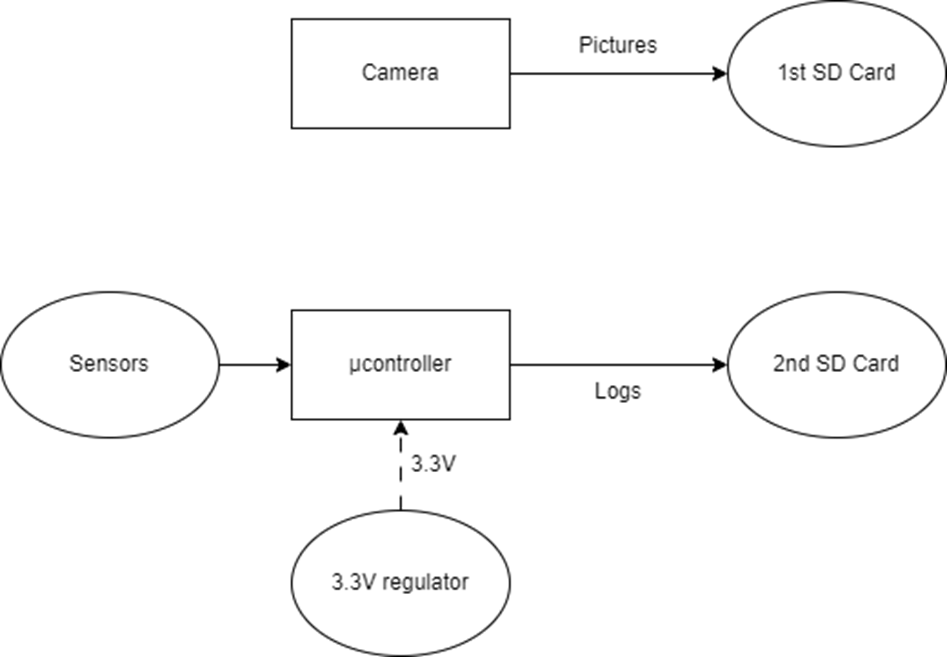
\includegraphics[width=0.9\textwidth]{\currfiledir/figures/storage_diagram.png}
    \caption{Storage system diagram}
\end{figure}
The storage system is made of a SD card linked to the camera and a second SD card linked to the microcontroller. The first SD card linked to the camera is used to store the pictures taken by the camera. The second one is used to store the logs emitted by the system.
The measures gathered by the sensors are fetched by the microcontroller, which sends them via LoRa to the gateway and stores them at the same time in the 2nd SD card.
\newpage
\subsection{The sensors}
\begin{figure}[!h]
    \centering
    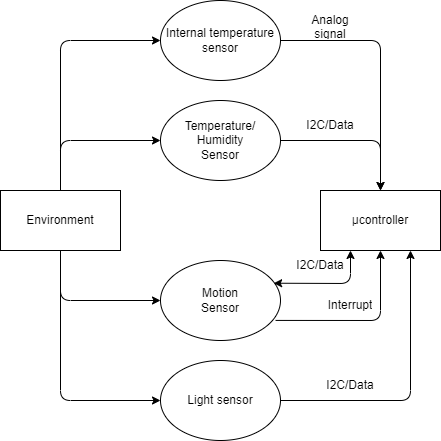
\includegraphics[width=0.8\textwidth]{\currfiledir/figures/sensor_diagram.png}
    \caption{Architecture diagram of the sensors and their relationship to other components}
\end{figure}

\noindent Our aim was to ultimately add sensors to the system in order to send information about it with the LoRa communication protocol. The researchers can then know the state of the system in real time, in order to not lose days or even weeks of pictures collected if the system has a problem.\\
In fact, the environment could perturbate the environment in 2 different ways:\\
The system could move (because of wind or potentially animals), which would unbalance the system. The system could then fall on the ground or take pictures of the wrong place. The researchers not knowing it could let the system in place during months, which could lead to a loss of time in their work.\\
The system could also be damaged by bad weather conditions, such as humidity and temperature. For example, if the temperature rises too much, the battery and other components could be damaged. So, it is important to detect the problems to inform the researchers.\\
The sensors would collect data in the environment and send it to the microcontroller in order to process it and log it. Then, the data would be sent to the storage system.




\newpage
\subsubsection{Motion sensor}
The motion sensor employed in this device is an ICM-20602. This motion tracking device was chosen for its low power consumption (1.33mA in low power mode and 2.79mA when in low noise mode). The ICM-20602 is also programmable, allowing users to define a threshold value to wake up the microcontroller.
For communication, the ICM-20602 utilizes an I2C interface, as well as an interrupt pin to signal events such as data-ready or wake-on-motion. This makes it easy to interface with a microcontroller and manage the sensor's operation.
The output data rate (ODR) for both the accelerometer and gyroscope can be configured based on your application requirements. When using interrupt-driven data collection, the interrupt pin can be set to trigger when new data is available, allowing the microcontroller to process the information.

\begin{figure}[!h]
    \centering
    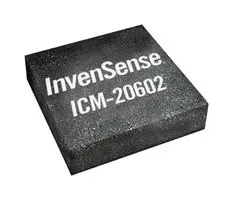
\includegraphics[width=0.4\textwidth]{\currfiledir/figures/20602.png}
    \caption{Picture of the motion sensor ICM-20602}
    \cite{20602}
\end{figure}

\newpage
\subsubsection{Humidity/Temperature sensor}
The AM2320 has been selected as the humidity and temperature sensor for this project due to its affordability and low power consumption (maximum 1mA and 50µA in sleep mode). This sensor covers a wide temperature range from -40 to 80°C and is capable of measuring humidity from 0 to 99.9\% relative humidity. The AM2320 is also equipped with an I2C connection, making it convenient for integration with a microcontroller.
In this application, humidity and temperature will be measured every 30 minutes. The I2C interface of the AM2320 facilitates communication with the microcontroller, allowing for efficient and accurate data collection at regular intervals. This ensures that the project remains energy-efficient while providing reliable temperature and humidity measurements.

%: Picture of the temperature and humidity sensor AM2320.
\begin{figure}[!h]
    \centering
    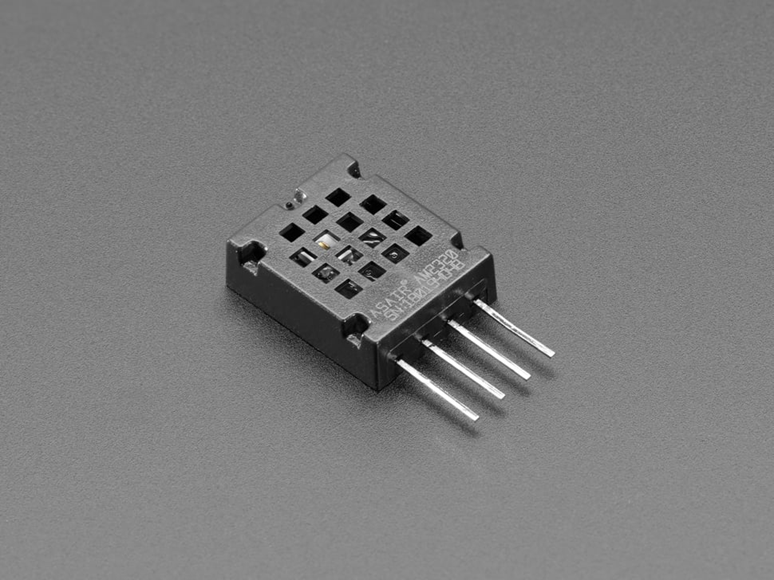
\includegraphics[width=0.4\textwidth]{\currfiledir/figures/AM2320.png}
    \caption{Picture of the temperature and humidity sensor AM2320}
    \cite{AM2320}
\end{figure}


\subsubsection{Temperature sensors}
The LM35DZ temperature sensor is selected for internal case temperature monitoring due to its high accuracy, low power consumption (less than 60µA), and easy interfacing with a microcontroller. It provides a linear output (10mV/°C), operates in a -55 to 150°C range, and minimizes self-heating, which reduces measurement interference. Temperature measurements will be taken every 30 minutes, ensuring energy-efficient and reliable monitoring.
\begin{figure}[!h]
    \centering
    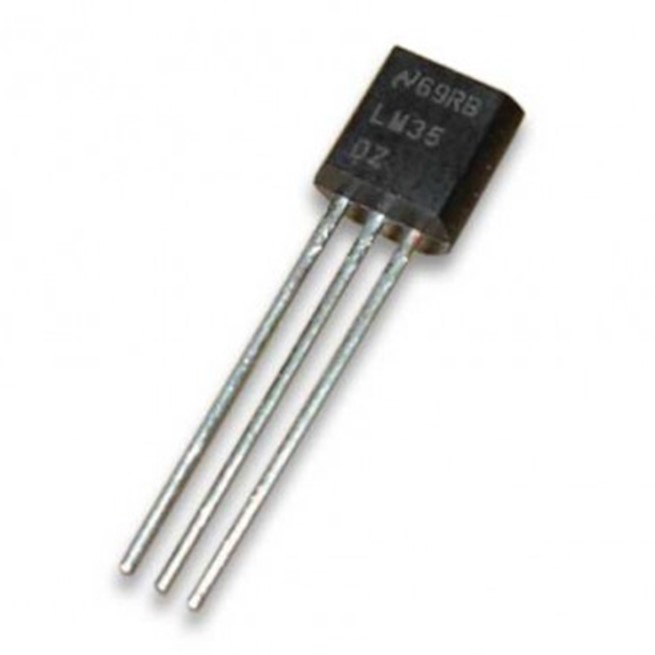
\includegraphics[width=0.25\textwidth]{\currfiledir/figures/LM35DZ.jpg}
    \caption{Temperature sensors LM35DZ}
    \cite{Temp}
\end{figure}



\newpage
\subsubsection{Light sensor}
For light sensing requirements, the chosen sensor is the TSL2561. This efficient and cost-effective sensor is known for its reliable light intensity measurements across a wide range of conditions. One of the key reasons for selecting the TSL2561 is its low power consumption, with a typical active current of 0.24mA and a power-down current of 2µA, which aligns with the project's focus on energy efficiency. Additionally, the sensor boasts a range of 0.1 to 40,000 lux, making it suitable for various lighting environments. The availability of the TSL2561 for quick delivery further contributed to this decision. Its I2C interface enables integration with the microcontroller, while the high-resolution 16-bit digital output ensures accurate and precise light readings.
In this application, the TSL2561 operates with an I2C interface and takes light measurements every 30 minutes. Additionally, a measurement is taken before capturing a photo to ensure optimal lighting conditions. This approach guarantees energy-efficient and precise light readings, contributing to the overall effectiveness of the project.
\begin{figure}[!h]
    \centering
    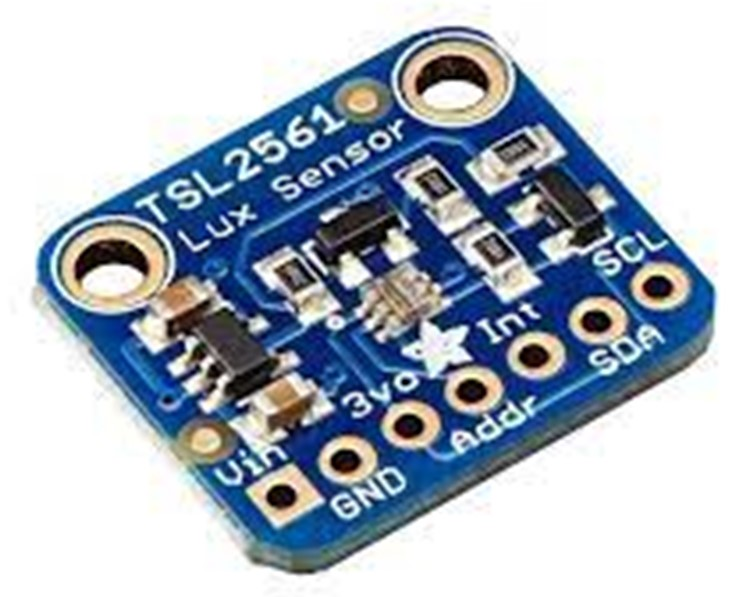
\includegraphics[width=0.4\textwidth]{\currfiledir/figures/TSL2561.jpg}
    \caption{TSL 2561}
    \cite{Light}
\end{figure}